\documentclass[11pt]{report}
\usepackage{mathrsfs,graphicx}
\begin{document}

\noindent
George Weigt

\noindent
Homework \#2

\bigskip
\noindent
{\bf 1.} Write the differential equation for the following system.
$${C(s)\over R(s)}={
s^4+2s^3+5s^2+s+1
\over
s^6+7s^5+3s^4+2s^3+s^2+3
}$$

\bigskip
\noindent
See Ogata p. 55.
We have $n=\mathop{\rm deg} R=6$ and $m=\mathop{\rm deg} C=4$ with
$n\ge m$ as required.
Hence
$$a_0,\ldots,a_n=1,7,3,2,0,3\qquad b_0,\ldots,b_m=1,2,5,1,1$$
and the differential equation is
$$
{d^6y\over dt^6}+
7{d^5y\over dt^5}+
3{d^4y\over dt^4}+
2{d^3y\over dt^3}+
{d^2y\over dt^2}+
3y=
{d^4x\over dt^4}+
2{d^3x\over dt^3}+
5{d^2x\over dt^2}+
{dx\over dy}+
x
$$

\newpage

\noindent
{\bf 2.} Find the transfer function for the following network.
\begin{center}
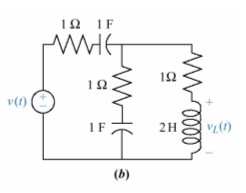
\includegraphics[scale=0.5]{images/210-1.png}
\end{center}

\bigskip
\noindent
The equation for the loop on the left:
$$1I_1(s)+{1\over s}I_1(s)+1I_1(s)+{1\over s}I_1(s)-1I_2(s)-{1\over s}I_2(s)=V(s)$$
The equation for the loop on the right:
$$1I_2(s)+2sI_2(s)+{1\over s}I_2(s)+1I_2(s)-1I_1(s)-{1\over s}I_1(s)=0$$
Hence
$$\left[\matrix{
2+2/s & -1-1/s\cr
-1-1/s & 2s+2+1/s\cr
}\right]
\left[\matrix{I_1(s) \cr I_2(s)}\right]
=\left[\matrix{V(s) \cr 0}\right]
$$
Solving for $I_2(s)$ we have
$$I_2(s)={(s^2+s)V(s)\over 4s^3+7s^2+4s+1}$$
The transfer function is
$${V_L(s)\over V(s)}={2sI_2(s)\over V(s)}=
{2s^3+2s^2\over 4s^3+7s^2+4s+1}$$

\end{document}
